\documentclass{article}
\usepackage[utf8]{inputenc}
\usepackage[T1]{fontenc}
\usepackage{lipsum}
\usepackage{graphicx}
\usepackage{amsmath}
\usepackage[margin=1in]{geometry}
\usepackage{titlesec}
\usepackage{enumitem}
\usepackage{geometry}
\usepackage{tabularx}
\usepackage{caption}
\usepackage{fixltx2e}
\usepackage{booktabs}
\usepackage{float}  

\titleformat{\section}
{\LARGE\bfseries}{\thesection}{1em}{}

\titleformat{\subsection}
{\Large\bfseries}{\thesection}{1em}{}

\begin{document}

\setcounter{subsection}{0}

\pagestyle{empty}

\newgeometry{left=2cm, right=2cm}
\begin{titlepage}
\begin{center}
    {{\Large{\textsc{Alma Mater Studiorum - Università di Bologna}}}}
    \rule[0.1cm]{\textwidth}{0.1px}
    \rule[0.5cm]{\textwidth}{0.6px}\\
    {\fontsize{12}{13}{SCUOLA DI SCIENZE \\ Corso di Laurea in Informatica per il Management}}
\end{center}

\vspace{50px}

\begin{center}
    {\LARGE{{\bf Piattaforma ESQL}}}\\
\end{center}

\vspace{115px}
\par
\noindent
\begin{minipage}[t]{0.04\textwidth}
~
\end{minipage}
\begin{minipage}[t]{0.4\textwidth}
\end{minipage}
\hfill
\begin{minipage}[t]{0.4\textwidth}\raggedleft
{\fontsize{12}{13}{SVOLTA DA:}\\
\fontsize{12}{13}{\it Canghiari Matteo \\ De Rosa Davide \\ Nadifi Ossama}}
\end{minipage}
\begin{minipage}[t]{0.04\textwidth}
~
\end{minipage}

\vspace*{210px}

\begin{center}
    \large{Anno Accademico 2023/2024}
\end{center}
\end{titlepage}

\subsection{Analisi dei requisiti}
\large
All'interno di questa prima sezione, si adotta un approccio orientato ad un'analisi degli aspetti principali inerenti al progetto, mediante una serie di azioni mirate per rendere il più comprensibile possibile il documento di specifica, attraverso la scelta del corretto livello di astrazione, la standardizzazione della struttura delle frasi oppure tramite la decomposizione del testo in espressioni omogenee. \vspace*{7px}\\
Di seguito sono descritti i concetti essenziali riferiti a ciascuna entità, affinchè sia definito un supporto concreto per successive fasi di sviluppo:
\begin{itemize}[label={-}]
    \itemsep0em
    \item 
\end{itemize}


\subsection{Progettazione concettuale}
\large
\subsubsection*{Modello E-R}
\begin{figure}[H]
    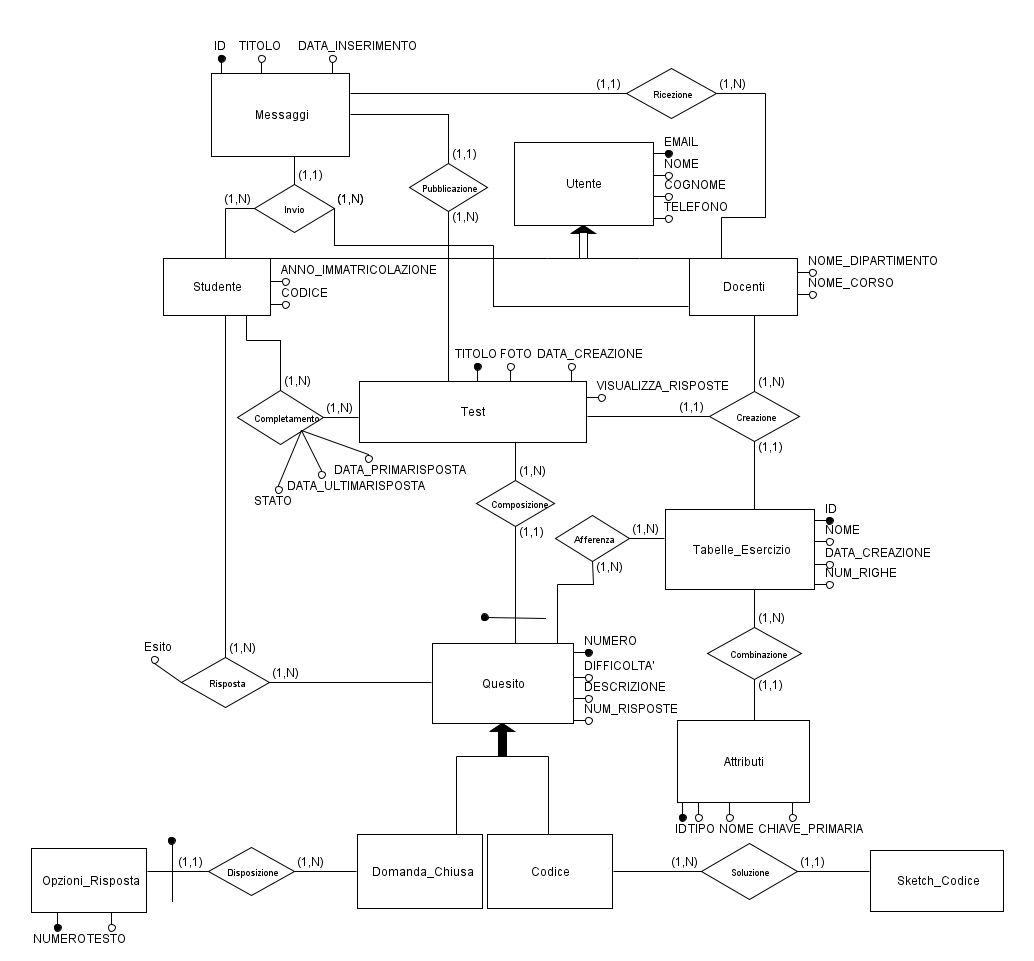
\includegraphics[width=1\textwidth]{foto1.png}
    \caption{Modello E-R precedente alla raffinazione.}
\end{figure}

\subsubsection*{Dizionario delle entità}
\begin{table}[H]
    \centering
    \begin{tabularx}{\textwidth}{|X|p{5cm}|p{5cm}|X|}
        \hline
        Entità & Descrizione & Attributi & Identificatore \\
        \hline
        Utente & Utilizzatore dell'applicativo & Email, Nome, Cognome, Telefono & Email \\        
        \hline
        Docenti & Docente creatore e ideatore di quesiti e tabelle di esercizio & Nome\_Dipartimento, Nome\_Corso & Email \\
        \hline
        Studente & Alunno che interagisce con l'applicativo per la risoluzione dei quesiti posti & Anno\_Ipxatricolazione, Codice & Email \\
        \hline
        Tabelle\_Esercizio & Tabelle che costituiscono parte dei meta-dati per la realizzazione di test & ID, Nome, Data\_Creazione, Num\_Righe & ID \\
        \hline
        Attributi & Attributi i quali costituiscono la seconda entità essenziale per i meta-dati, legati alla realizzazione di test da sopxinistrare & ID, Tipo Nome, Chiave\_Primaria & ID \\
        \hline
        Test & Test indica l'insieme di quesiti svolti dagli studenti e creati dal docente & Titolo, Foto, Data\_Creazione, Visualizza\_Risposte & Titolo \\
        \hline
        Quesito & Domanda relativa a tematiche svolte nel corso & Numero, Difficoltà, Descrizione, Num\_Risposte & Numero \\
        \hline
        Domanda\_Chiusa & Tipologia di Quesito, rappresentante una domanda a scelta multipla & . & Numero \\
        \hline
        Sketch\_Codice & Tipologia di Quesito, richiedente la formulazione di query SQL & . & Numero \\
        \hline
        Messaggi & Comunicazioni ricevute e inviate tra docenti e studenti & ID, Titolo, Data\_Inserimento & ID \\
        \hline
    \end{tabularx}
    \caption{Descrizione delle entità del modello E-R precedente alla raffinazione.}
\end{table}

\subsubsection*{Dizionario delle relazioni}
\begin{table}[H]
    \centering
    \begin{tabularx}{\textwidth}{|X|p{5cm}|p{3cm}|X|}
        \hline
        Relazione & Descrizione & Componenti & Attributi \\
        \hline
        Creazione & Creazione da parte di docenti di tabelle di esercizio e quesiti & Docenti, Tabelle\_Esercizio, Test & . \\
        \hline
        Completamento & Completamento di un test sopxinistrato da parte degli studenti & Studente, Test & Stato, Data\_UltimaRisposta, Data\_PrimaRisposta \\
        \hline
        Invio & Invio di messaggi da parte di docenti e studenti & Studente, Docenti, Messaggi & . \\
        \hline 
        Pubblicazione & Pubblicazione di comunicazioni afferenti ad uno specifico test & Messaggi, Test & . \\
        \hline
        Ricezione & Ricezione di messaggi emessi da studenti oppure da docenti & Messaggi, Docenti & . \\
        \hline
        Risposta & Risposta formulata dagli studenti in relazione ad uno specifico quesito & Studente, Quesito & Esito \\
        \hline
        Composizione & Composizione di un insieme di quesiti rispetto ad un determinato test & Quesito, Test & . \\
        \hline
        Afferenza & Afferenza dei quesiti ideati relativamente a tabelle di esercizio & Quesito, Tabelle\_Esercizio & . \\
        \hline
        Combinazione & Combinazione di attributi per la costruzione di tabelle di esercizio & Tabelle\_Esercizio, Attributi & . \\
        \hline
        Soluzione & Soluzione alla query SQL richiesta & Codice, Skecth\_Codice & . \\
        \hline
        Disposizione & Disposizione del numero complessivo di opzioni di risposta relative alla domanda sottoposta & Domanda\_Chiusa, Opzioni\_Risposta & . \\    
        \hline
    \end{tabularx}
    \caption{Descrizione delle relazioni del modello E-R precedente alla raffinazione.}
\end{table}

\subsubsection*{Modello E-R raffinato}
\begin{figure}[H]
    \includegraphics*[width=1.1\textwidth]{foto2.png}
    \caption{Modello E-R successivo alla raffinazione.}
\end{figure}

\subsection{Progettazione logica}
\large
\dots 

\subsection{Normalizzazione}
\large
\dots 

\subsection{Descrizione delle funzionalità}
\large
\dots 

\subsection{Codice SQL}
\large
\dots 


\subsubsection*{Costo operazionale}


\end{document}